\chapter{Question 1}
\label{question-1}
\section{Question}

\begin{itemize}
\item Using the pages from A3 that boilerpipe successfully processed, download those representations again \& reprocess them with boilerpipe.
\item Document the time difference (e.g., Time(A4) – Time(A3)).
\item Compute the Jaccard Distance x for each pair of pages (i.e., P(A3) \& P(A4) for:
	\begin{itemize}
		\item Unique terms (i.e., unigrams)
		\item Bigrams
		\item Trigrams
	\end{itemize}
\item See: \url{http://en.wikipedia.org/wiki/Jaccard_index}
\item For each of the 3 cases (i.e., 1-, 2-, 3-grams) build a Cumulative Distribution Function that shows the \% change on the x-axis \& the \% of the population on the x-axis 
\item See: \url{http://en.wikipedia.org/wiki/Cumulative_distribution_function}
\item Give 3-4 examples illustrating the range of change that you have measured.
\end{itemize}


\section{Solution}
\begin{itemize}
\item The time difference between the time since I ran the boilerpipe for the URIs for assignment three and assignment four was 30 days.
\item I used the same boilerpipe library as I used in assignment three.
\item From the 10000 URIs I ran through boilerpipe I was able to successfully retrieve the data from 6086 URIs.
\item I used the `ngrams' python library for fetching the unigrams, bigrams and trigrams. I used the set data structure to ensure that only the unique terms were included in the comparison.
\item The Jaccard Distance can be calculated by finding the union and the intersection. It is the ratio of the difference of the union and intersection by the union of the set.
\item Below are the graphs for unigrams, bigrams and trigrams.
\end{itemize}

	\begin{minipage}{\linewidth}
		\centering
			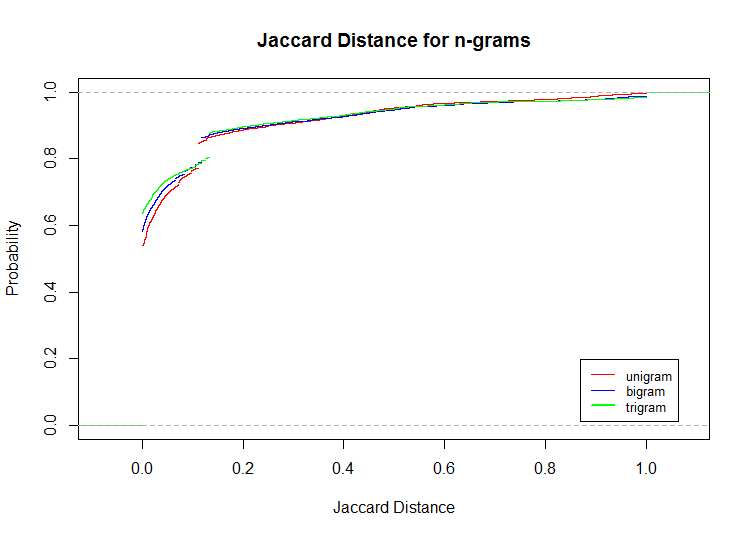
\includegraphics[scale=0.55]{figures/q1/ngram}
		\captionof{figure}{CDF - Jaccard Distance vs. Probability}
		\label{wordCount}
	\end{minipage}
	
	\begin{minipage}{\linewidth}
		\centering
			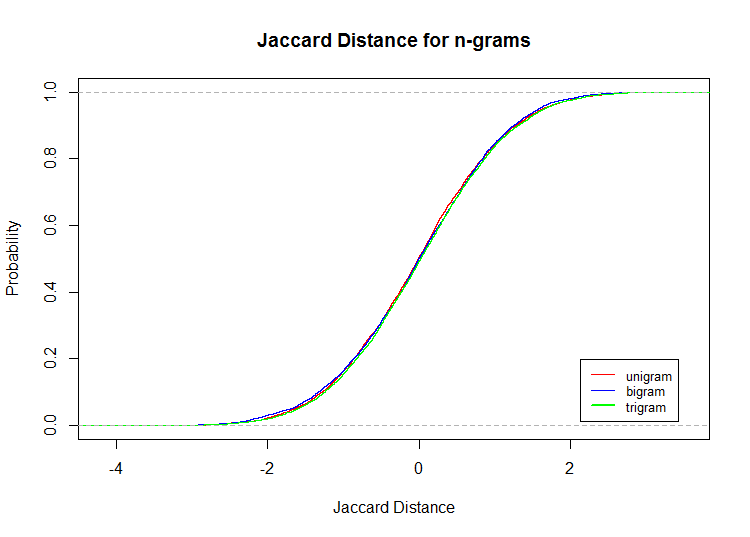
\includegraphics[scale=0.55]{figures/q1/ngram_normalized}
		\captionof{figure}{CDF normalized - Jaccard Distance vs. Probability}
		\label{wordCount}
	\end{minipage}

\newpage
\section{Code Listing}

\lstinputlisting[language=Python,breaklines = true,frame=single,caption={Python program for fetching the boilerpipe content from the URIs.},label=lst:q1-1,captionpos=b,numbers=left,showspaces=false,showstringspaces=false,basicstyle=\footnotesize]{pythonFiles/getBoilerPipe.py}

\newpage
\lstinputlisting[language=Python,breaklines = true,frame=single,caption={Python program for calculating the Jaccard Distance.},label=lst:q1-1,captionpos=b,numbers=left,showspaces=false,showstringspaces=false,basicstyle=\footnotesize]{pythonFiles/getNGrams.py}

\newpage
\lstinputlisting[language=R,breaklines = true,frame=single,caption={R program for generating the CDF for Jaccard Distance.}, label=lst:q1R1,captionpos=b,numbers=left,showspaces=false,showstringspaces=false,basicstyle=\footnotesize]{rFiles/cdfQ1.r}